\let\negmedspace\undefined
\let\negthickspace\undefined
\documentclass[journal]{IEEEtran}
\usepackage[a5paper, margin=10mm, onecolumn]{geometry}
%\usepackage{lmodern} % Ensure lmodern is loaded for pdflatex
\usepackage{tfrupee} % Include tfrupee package

\setlength{\headheight}{1cm} % Set the height of the header box
\setlength{\headsep}{0mm}     % Set the distance between the header box and the top of the text

\usepackage{gvv-book}
\usepackage{gvv}
\usepackage{cite}
\usepackage{amsmath,amssymb,amsfonts,amsthm}
\usepackage{algorithmic}
\usepackage{graphicx}
\usepackage{textcomp}
\usepackage{xcolor}
\usepackage{txfonts}
\usepackage{listings}
\usepackage{enumitem}
\usepackage{mathtools}
\usepackage{gensymb}
\usepackage{comment}
\usepackage[breaklinks=true]{hyperref}
\usepackage{tkz-euclide} 
\usepackage{listings}
% \usepackage{gvv}                                        
\def\inputGnumericTable{}                                 
\usepackage[latin1]{inputenc}                                
\usepackage{color}                                            
\usepackage{array}                                            
\usepackage{longtable}                                       
\usepackage{calc}                                             
\usepackage{multirow}                                         
\usepackage{hhline}                                           
\usepackage{ifthen}                                           
\usepackage{lscape}
\begin{document}

\bibliographystyle{IEEEtran}
\vspace{3cm}

\title{4.12.2}
\author{EE25BTECH11065 - Yoshita J}
% \maketitle
% \newpage
% \bigskip
{\let\newpage\relax\maketitle}

\renewcommand{\thefigure}{\theenumi}
\renewcommand{\thetable}{\theenumi}
\setlength{\intextsep}{10pt} % Space between text and floats

\textbf{Question}:\\
For which value of $k$ will the following pair of linear equations have no solution?
\begin{align*}
    3x + y &= 1 \\
    (2k - 1)x + (k - 1)y &= 2k + 1
\end{align*}
\bigskip

\textbf{Solution:} \\
The given system of equations is\\

\begin{table}[H]    
  \centering
  \begin{tabular}{|c|c|}
\hline
\textbf{Name} & \textbf{Value} \\ \hline
$\vec{A}$ & $\myvec{2 & 1 \\0 & 3}$ \\ \hline
\end{tabular}

  \caption{Answers}
  \label{Answers}
\end{table}
In matrix form:
\begin{align}
\myvec{3 & 1 \\ 2k-1 & k-1}\myvec{x \\ y} = \myvec{1 \\ 2k+1}
\end{align}

Now, form the augmented matrix:
\begin{align}
\augvec{2}{1}{3 & 1 &  1 \\ 2k-1 & k-1 & 2k+1}
\end{align}

Perform row reduction:
\begin{align}
R_1 \to \tfrac{1}{3}R_1 
&\quad\Rightarrow\quad
\augvec{2}{1}{1 & \tfrac{1}{3} & \tfrac{1}{3} \\[6pt]
2k-1 & k-1 & 2k+1} \\[10pt]
%
R_2 \to R_2-(2k-1)R_1
&\quad\Rightarrow\quad
\augvec{2}{1}{1 & \tfrac{1}{3} & \tfrac{1}{3} \\[6pt]
0 & \tfrac{k-2}{3} & \tfrac{4k+4}{3}} \\[10pt]
%
R_2 \to \tfrac{3}{k-2}R_2
&\quad\Rightarrow\quad
\augvec{2}{1}{1 & \tfrac{1}{3} & \tfrac{1}{3} \\[6pt]
0 & 1 & \tfrac{4k+4}{k-2}} \\[10pt]
%
R_1 \to R_1-\tfrac{1}{3}R_2
&\quad\Rightarrow\quad
\augvec{2}{1}{1 & 0 & \tfrac{1}{3}-\tfrac{1}{3}\cdot\tfrac{4k+4}{k-2} \\[6pt]
0 & 1 & \tfrac{4k+4}{k-2}}
\end{align}

For inconsistency, we need:
\begin{align}
k-2 = 0 \quad \text{and} \quad 4k+4 \neq 0
\end{align}
So,
\begin{align}
k = 2, \quad 4(2)+4 = 12 \neq 0
\end{align}

\begin{align*}
\boxed{k = 2}
\end{align*}
\newpage
\begin{figure}[h!]
\begin{center}
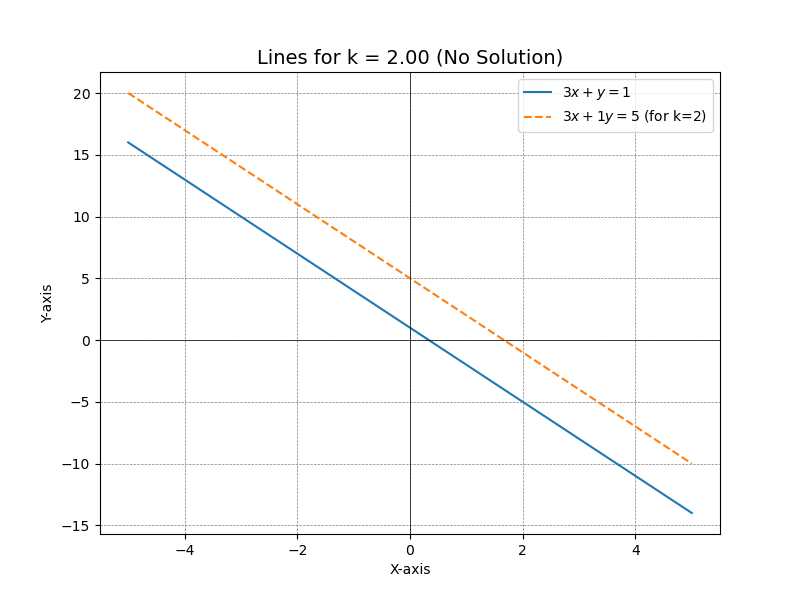
\includegraphics[width=\columnwidth]{figs/fig5.png}
\end{center}
\caption{A plane passing through point A with normal vector n.}
\label{fig:Fig.1}
\end{figure}
\end{document}




